%% ------------------------------------------------------------------- %%
%% ------------------------------------------------------------------- %%
%% ------------------------------------------------------------------- %%
%% ------------------------------------------------------------------- %%
\chapter{Marco Conceptual}
\label{cap:marcoteorico}

\lhead{\emph{Marco Conceptual}} 

El proyecto pertenece al área de Bioinformática y específicamente a la Inmunoinformática, en este contexto el marco teórico detalla conceptos de Biología Molecular (ADN, ARN y proteínas), Inmunología y Ciencias de la Computación. 

\section{Bioinformática y Biología Molecular }

En esta sección, describiremos los principales conceptos referentes a Biología Molecular que serán considerados en la propuesta de la tesis.

\subsection{Bioinformática}

Según \cite{luscombe2001bioinformatics}, la Bioinformática involucra la tecnología que utiliza las computadoras para el almacenamiento, manipulación y distribución de información relacionada a la Biología Molecular como DNA, RNA y proteínas. También podemos considerar que la Bioinformática se enfoca al análisis de secuencias, estructuras y funciones de los genes y proteínas; algunas veces también puede ser llamado Computación Molecular Biológica \citep{xiong2006essential}.


\subsubsection{DNA, RNA y Proteínas}

\textit{Deoxyribonucleic Acid} (DNA) es una molécula dentro de las células que contiene información genética responsable del desarrollo y función del organismo \citep{NCIdictionary2022}. Gran parte del DNA se sitúa dentro del núcleo de las células (en organismos Eucariotes). Por ejemplo en la Figura \ref{img:dnalocation}, vemos como el DNA, forma parte de los cromosomas y estos a su vez están en el núcleo. Luego, podemos notar, que los genes representan segmentos del DNA. Finalmente, en la Figura \ref{img:dnalocation}, notamos las bases nitrogenadas que componen el DNA: \textit{Guanine}, \textit{Cytosine}, \textit{Adenine} y \textit{Thymine}; normalmente, estas bases serán representadas por las letras: G, C, A, T respectivamente.

\begin{figure}[H]
	\centering
	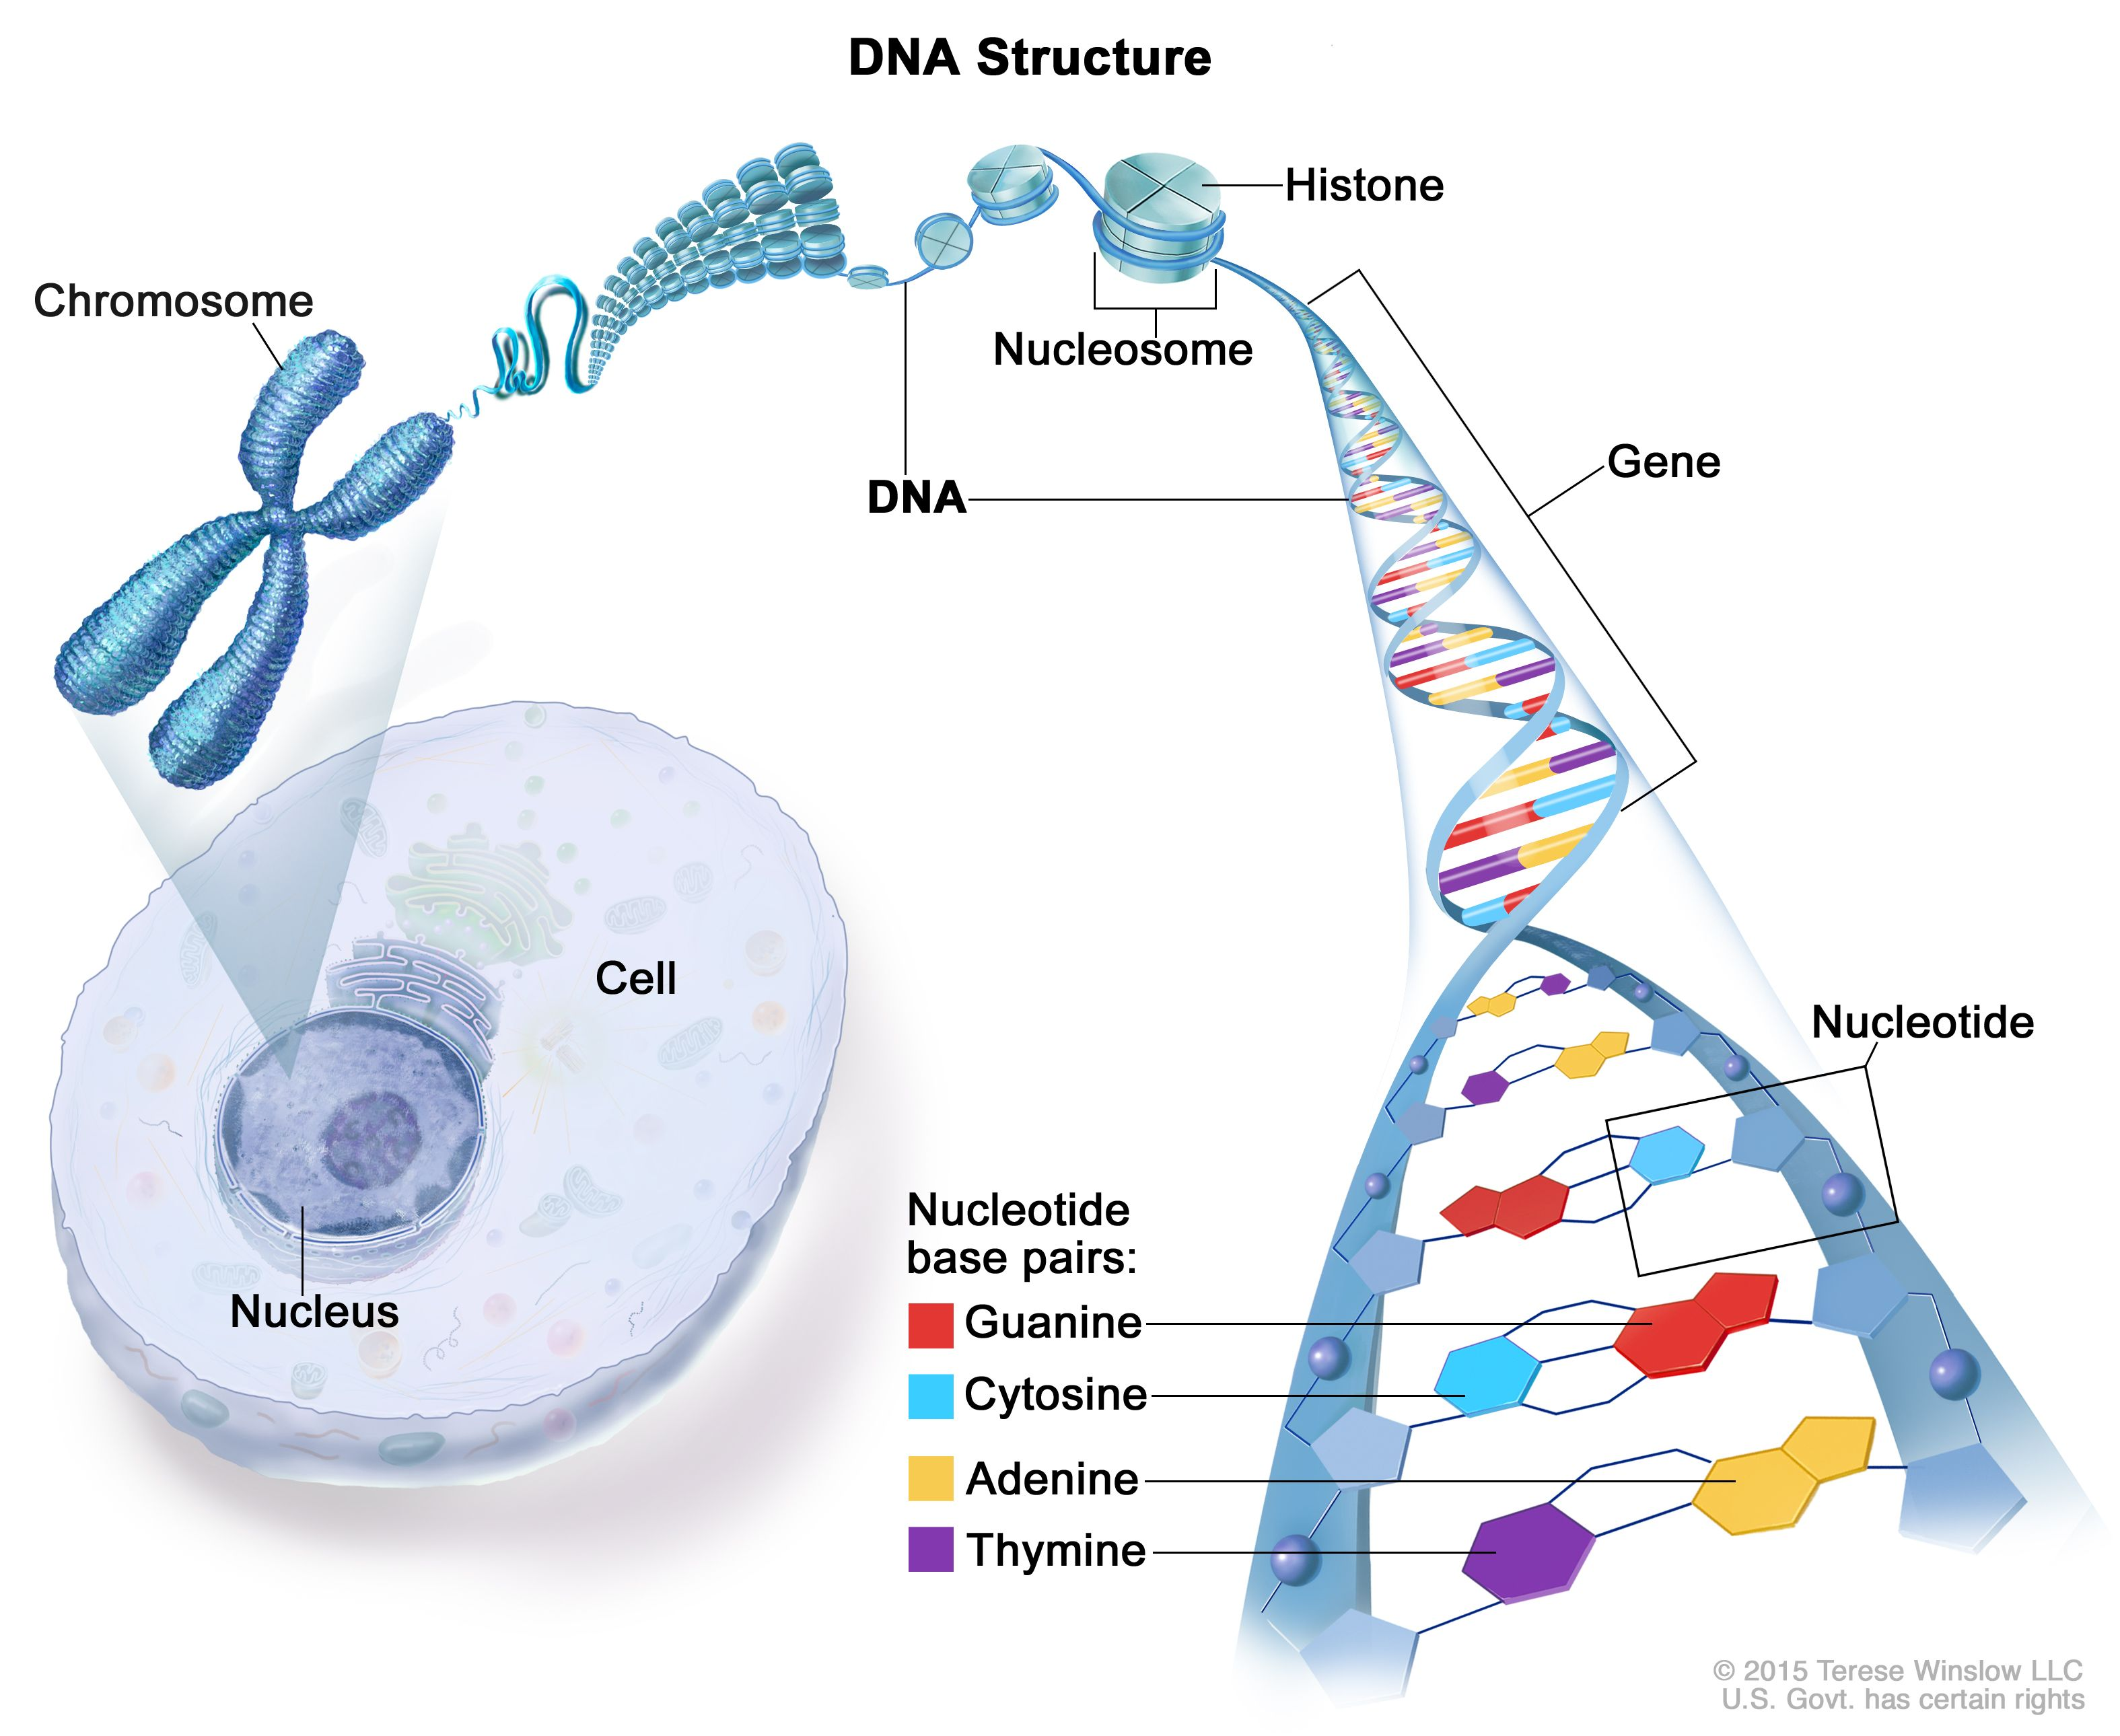
\includegraphics[width=0.6\textwidth]{img/neoantigen/dna}
	\caption{Localización y estructura del DNA. Fuente:  \cite{NCIdictionary2022}.}	
	\label{img:dnalocation}
\end{figure}

Durante el ciclo de vida de la célula, ocurre un proceso llamado Transcripción (ver Figura \ref{img:trans}), en este proceso se generan cadenas de \textit{Ribonucleic Acid} (RNA) a partir de la cadena de DNA \citep{NCIdictionary2022}.  Durante este proceso la base nitrogenada \textit{Thymine} (T) es reemplazada por \textit{Uracil} (U). El proceso mencionado, ocurre dentro del núcleo de la célula y en esta etapa el RNA es llamado \textit{messenger RNA} (mRNA). Una vez el mRNA sale del núcleo, es transportado por \textit{transfer RNA} (tRNA) hacia los Ribosomas (ver Figura \ref{img:trans}). En está, última etapa ocurre la Traducción, cada grupo de tres bases nitrogenadas (codones) se convierten en un aminoácido diferente, luego estos aminoácidos forman cadenas polipeptídicas y estas a su vez forman las proteínas; normalmente, cada gen genera una proteína \citep{xiong2006essential, NCIdictionary2022}.



\begin{figure}[H]
	\centering
	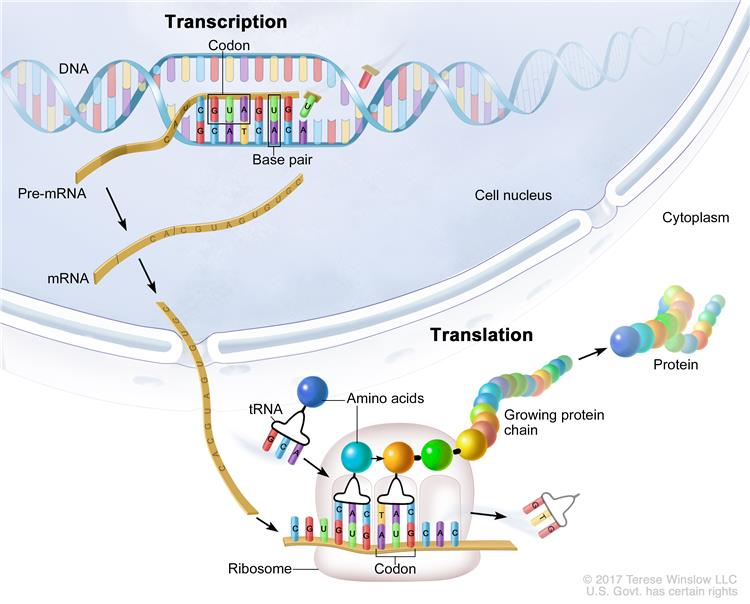
\includegraphics[width=0.7\textwidth]{img/neoantigen/trans}
	\caption{Transcripción y traducción. Fuente:  \cite{nci2020}.}	
	\label{img:trans}
\end{figure}

Durante el proceso de Traducción, puede ocurrir un fenómeno llamado \textit{Alternative Splicing}. Por ejemplo , en la Figura \ref{img:alt}, notamos como un gen puede generar tres proteínas distintas, cada una con funciones distintas. Este fenómenos, complica bastante el análisis de DNA.


\begin{figure}[H]
	\centering
	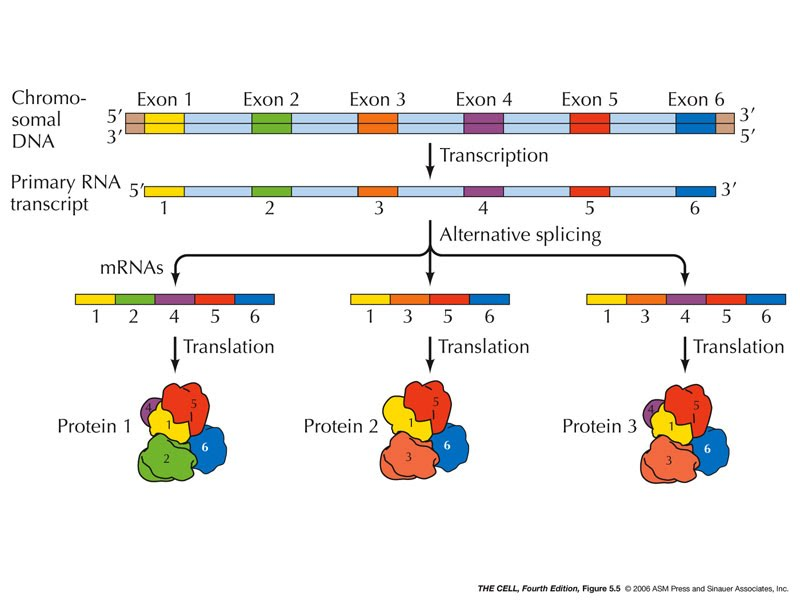
\includegraphics[width=0.7\textwidth]{img/neoantigen/alt}
	\caption{\textit{Alternative Splicing}. Fuente:  \cite{nci2020}.}	
	\label{img:alt}
\end{figure}


\subsection{Mutaciones}

Las mutaciones también llamadas variaciones, representan cualquier cambio en la secuencia de DNA, estos pueden ocurrir durante la división celular o por la exposición a agentes químicos o radioactivos. Estas mutaciones pueden ser beneficiosas, dañinas (cuando afectan la generación de proteínas) o no tener algún efecto  \citep{NCIdictionary2022}. Varios tipos de Cáncer son ocasionados por estas mutaciones \citep{borden2022cancer, chen2021challenges, de2020neoantigen}. \\ 

Según el tipo de célula afectada, tenemos: mutaciones somáticas y mutaciones \textit{germline} (una mutación en estas células puede ser heredada a la descendencia) \citep{clancy2008genetic}.  Según \citep{xu2018review}, las variaciones genómicas pueden clasificarse en tres grupos: \textit{Single-Nucleotide Variant} (SNV), inserciones y eliminaciones (INDELS) y \textit{Structural Variation} (SV). Una mutación se considera SNV cuando las variaciones afectan a menos de 10 bases. \\

En la Figura \ref{fig:SNV}, presentamos ejemplos de SNV. Por ejemplo, las sustituciones pueden afectar la generación de un aminoácido, pero las inserciones o eliminaciones pueden afectar en cadena la generación de varios aminoácidos, a este tipo de fenómeno se le conoce como \textit{frameshit mutation} \citep{xu2018review}.


\begin{figure}[h]
	\centering
	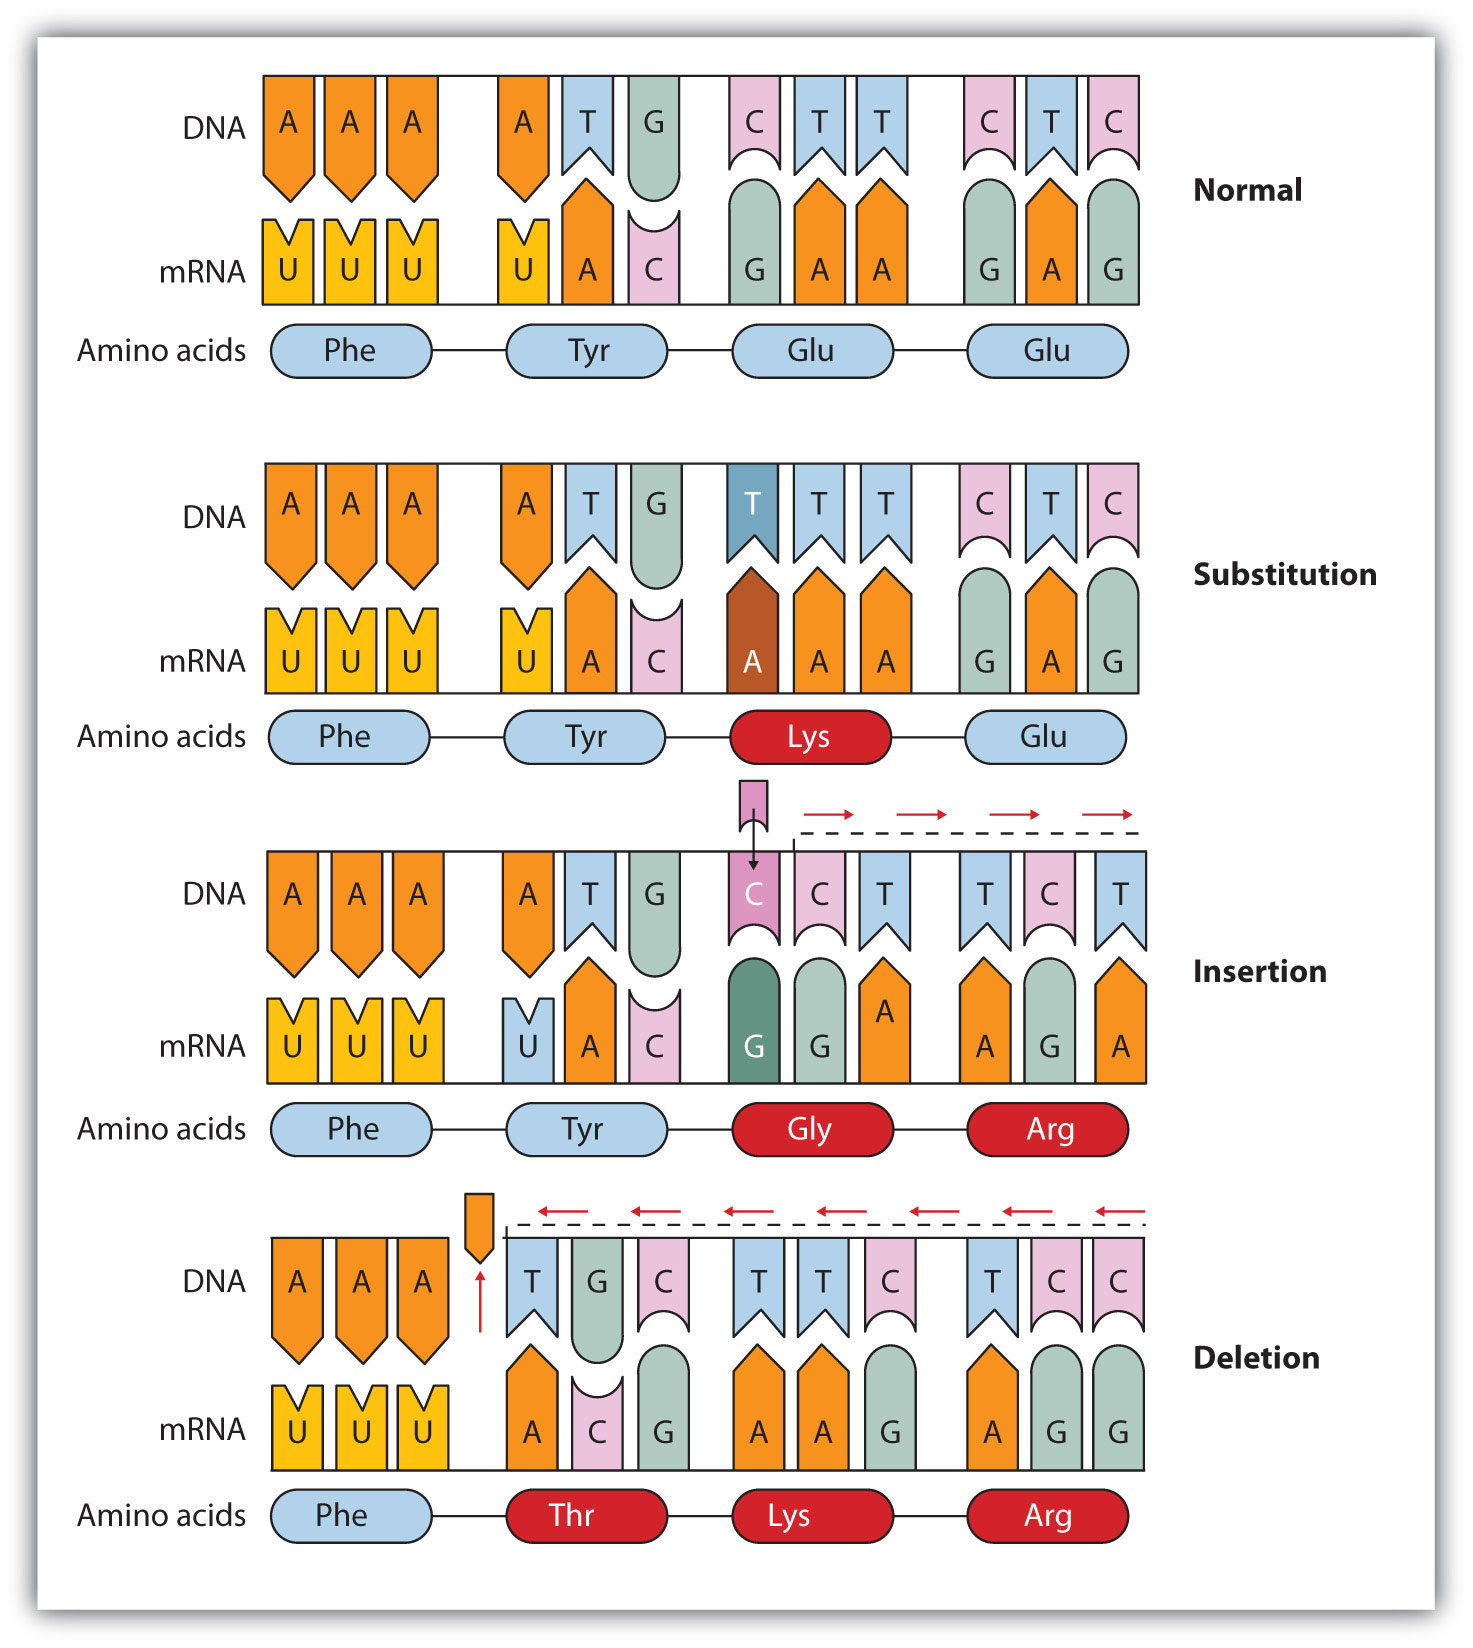
\includegraphics[width=0.6\textwidth]{img/neoantigen/SNV}
	\caption{Ejemplos de SNV en el DNA. Fuente: \cite{socrates2022}}
	\label{fig:SNV}
\end{figure}

En la Figura \ref{fig:variants}, mostramos algunos tipos de SV. En este caso, también se pueden presentar INDELS, \textit{Tanden duplication}, inversiones, traslocaciones y \textit{Copy Number Variants} (CNV). Los CNVs, representan fuertes candidatos para ser biomarcadores de varios tipos de Cáncer \citep{pan2019identification, lucito2007copy}. Otra mutación importante, es referente a la fusión de genes, en estos casos dos o más genes se fusionan y forman una proteína completamente diferente, este tipo de mutación también está fuertemente relacionado a varios tipos de Cáncer \citep{kerbs2022fusion, kim2019fusiongdb, heyer2020sequencing}.

\begin{figure}[h]
	\centering
	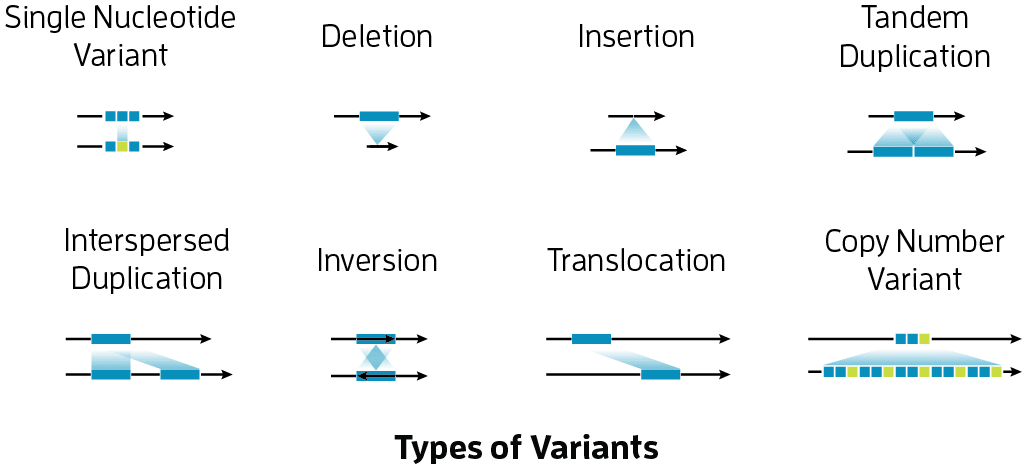
\includegraphics[width=0.6\textwidth]{img/neoantigen/variants}
	\caption{Ejemplos de variaciones en el DNA. Fuente: \cite{sv_pacbio_2021}}
	\label{fig:variants}
\end{figure}

\section{Sistema inmunitario}

El sistema inmunitario hace referencia al conjunto de células y procesos químicos que tiene como función protegernos de agentes extraños como: microbios, bacterias, células de Cáncer, toxinas, etc. \cite{marshall2018introduction}. En esta sección, se explicará de forma breve el comportamiento del sistema inmunitario frente cuando un agente extraño (antígeno) ingresa al cuerpo humano.

\subsection{Células T y APC}

Las células T también llamadas linfocitos T, se forman a partir de la médula ósea y son los encargados de eliminar agentes extraños (antígenos) \cite{NCIdictionary2022}. Estas células están compuestas por un T-cell Receptor (TCR), que es el encargado de reconocer y enlazar a los antígenos. Luego, algunas células T, requieren de la acción de los \textit{Antigen Presenting Cells} (APC), estás células APC son: células dentríticas, macrofagos, células B, fibroblastos y células epiteliales. Normalmente, los APC devoran los antígenos y luego los presentan a las células T para su eliminación  \citep{marshall2018introduction}.


\subsection{MHC I y II}

\textit{Major Histocompatibility Complex} (MHC) I y II, son proteínas que desempeñan un rol importante en el sistema inmunitario. Ambas proteínas tienen la función de presentar péptidos (antígenos) en la superficie de las células, para que sean reconocidas por la células T \citep{abualrous2021major}. MHC-I se encarga de la presentación de las células con núcleo, mientras que MHC-II, de las células APC. \\

El proceso de presentación de los antígenos por MHC-I es el siguiente (Figura \ref{fig:mhc1}): la proteína foránea es degradado por el proteasoma y se producen péptidos (posibles antígenos), luego estos péptidos son transportados al Endoplasmic Reticulum (ER) con la ayuda de \textit{Transporter associated Antigen Processing} (TAP), luego es migrado al aparato de Golgi para ser presentado en la superficie de la célula y es enlazado a la proteína MHC-I, una vez en la superficie, el antígeno puede ser reconocido por las células CD8+T \citep{zhang2019application}.




\begin{figure}[H]
	\centering
	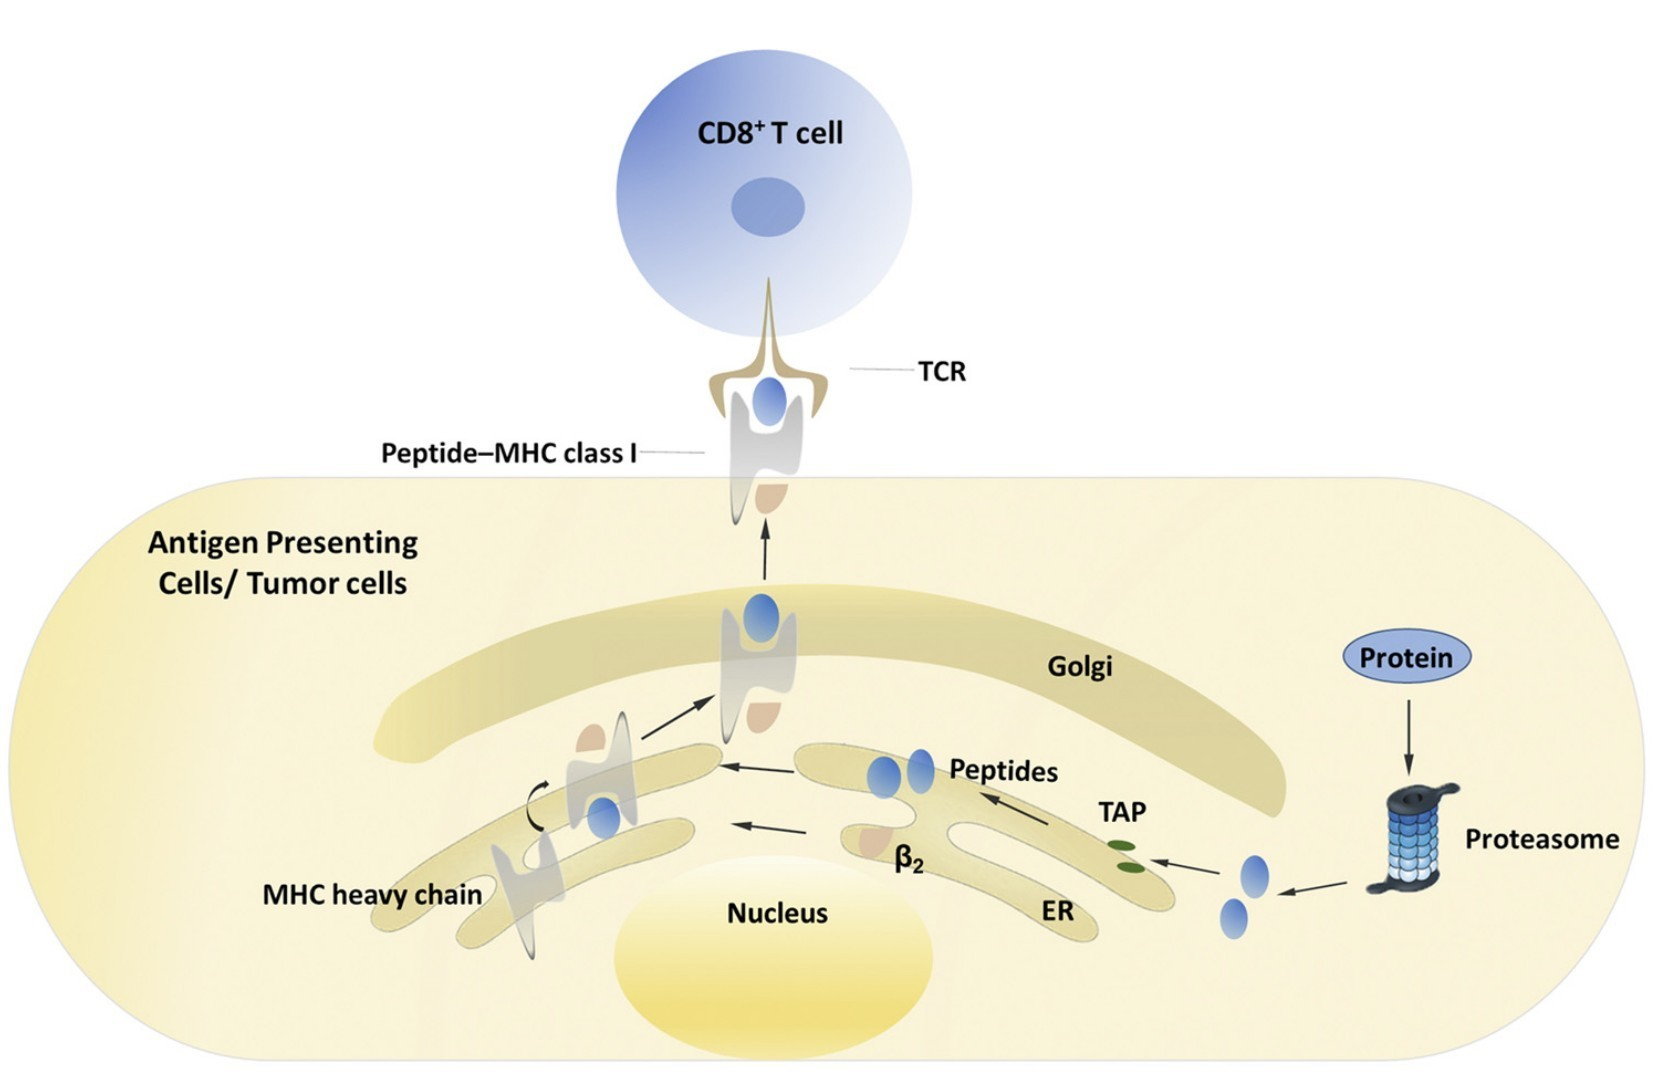
\includegraphics[width=0.8\textwidth]{img/neoantigen/mhc1.jpg}
	\caption{Presentación de antígenos por MHC-I. Fuente: \cite{zhang2019application}}
	\label{fig:mhc1}
\end{figure}

Para el caso de MHC-II, es un proceso similar (Figura \ref{fig:mhc2}): primero, los patógenos son devorados por fagocitosis, los péptidos asociados a MHC-II son producidos en el Endoplasmic Reticulum (ER), para luego ser trasladados al aparato de Golgi, y luego ser transportados a la superficie de las células una vez enlazadas con MHC-II, finalmente, son reconocidas por las células CD4+T \citep{zhang2019application}.



\begin{figure}[H]
	\centering
	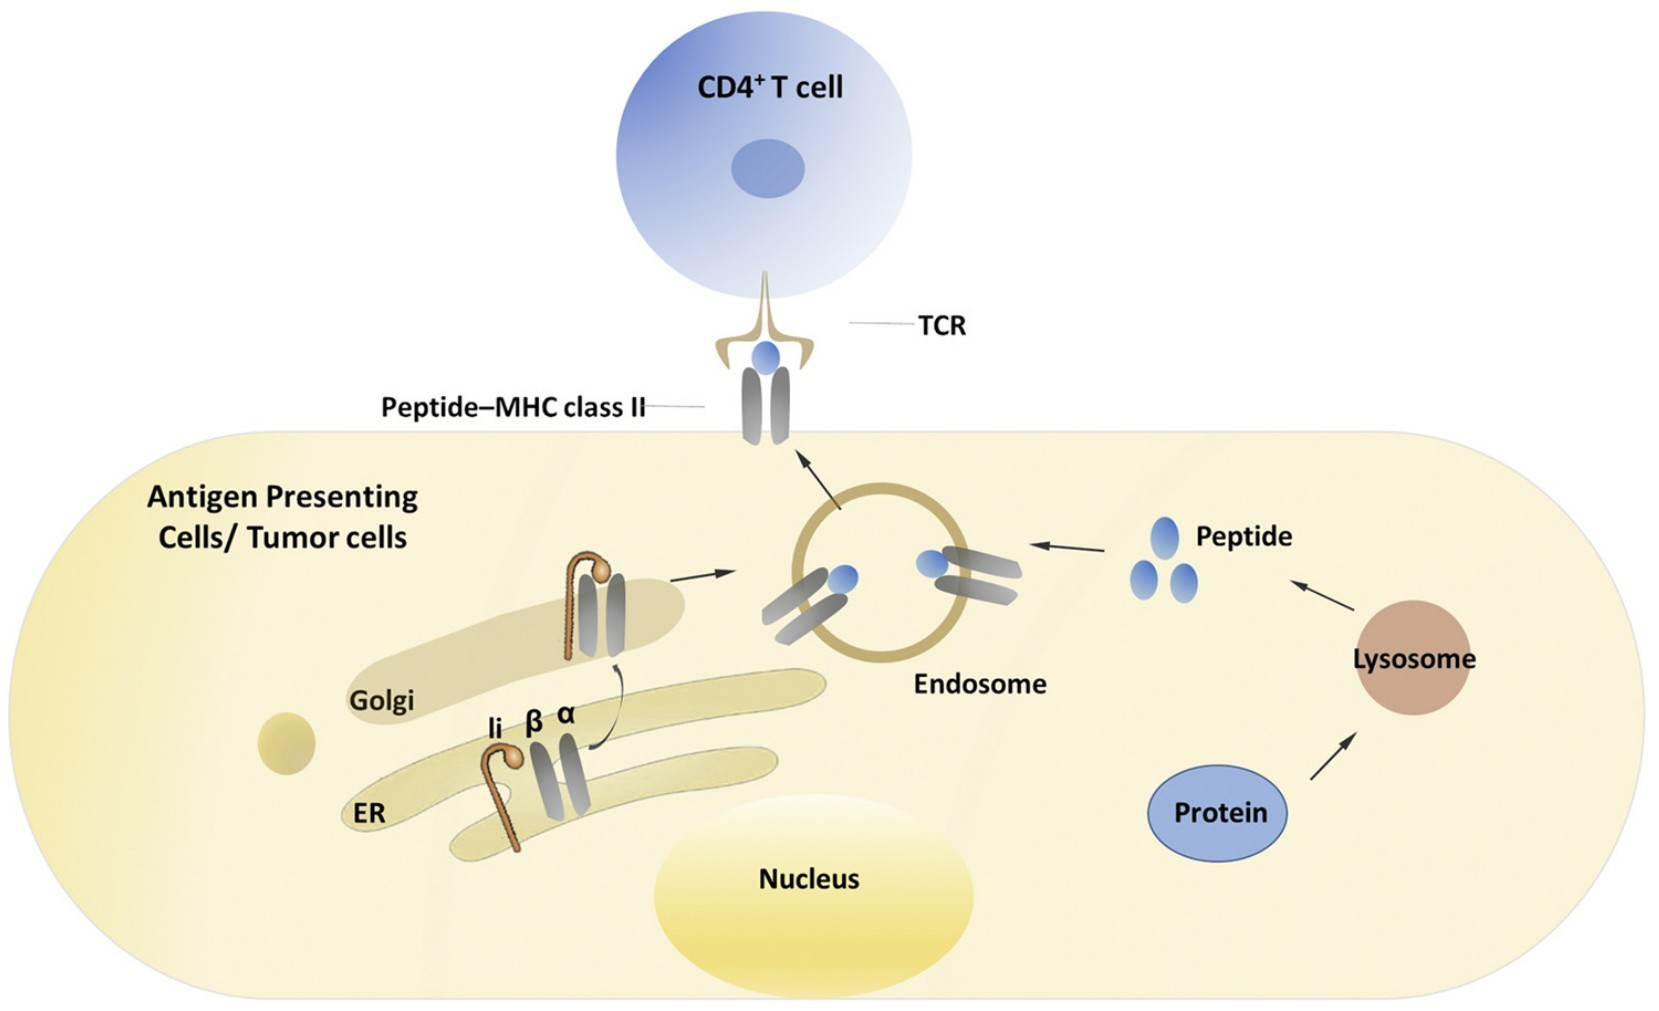
\includegraphics[width=0.8\textwidth]{img/neoantigen/mhc2.jpg}
	\caption{Presentación de antígenos por MHC-II. Fuente: \cite{zhang2019application}}
	\label{fig:mhc2}
\end{figure}

\subsection{Neo antígenos}

Es una proteína que se forma en las células de Cáncer cuando ocurre mutaciones en el DNA. Los neo antígenos cumplen un rol importante al estimular una respuesta inmune en contra de células de Cáncer. En la actualiadad, se estudia su uso en el desarrollo de vacunas contra el Cáncer \cite{NCIdictionary2022}. Una característica importante de los neo antígenos, es que solo están presentes en células tumorales y no en células sanas, debido a eso son considerados factores clave en la inmunoterapia del Cáncer \cite{borden2022cancer}. En la actualidad hay varios métodos para detectar a predecir neo antígenos, pero solo una pequeña porción de ellos logran estimular al sistema inmune \cite{chen2021challenges, hao2021improvement}.

 Este proceso para la detección de neo antígenos, generalmente consiste en: (1) extracción del tejido tumoral, (2) identificación de mutaciones, (3) detección de neo antígenos y predicción de inmunogenicidad, (4) desarrollo de experimentos in vitro y (5) desarrollo de la vacuna \citep{de2020neoantigen, peng2019neoantigen} (ver Figura \ref{fig:process}). \\

\begin{figure}[H]
	\centering
	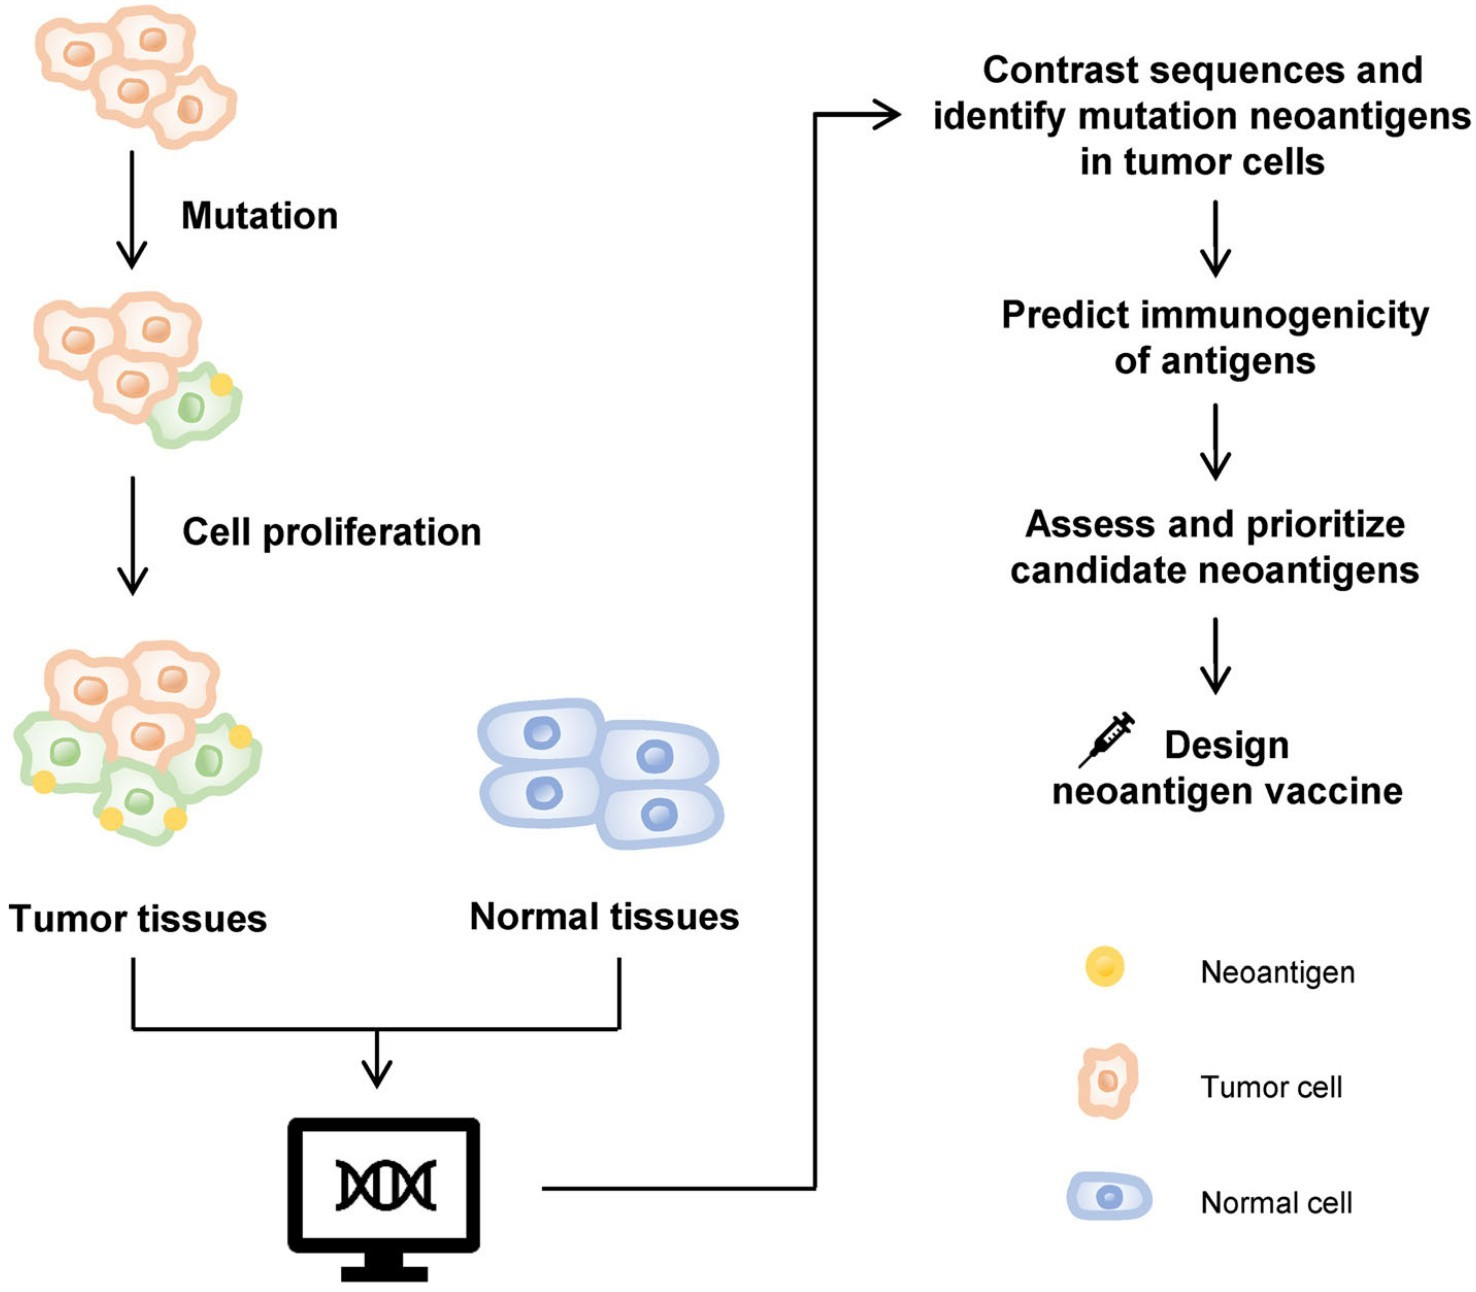
\includegraphics[width=0.7\textwidth]{img/neoantigen/process}	
	\caption{Proceso para la detección de neo antígenos y generación de vacunas personalizadas. Fuente: \citep{de2020neoantigen} }
	\label{fig:process}
\end{figure}


\section{\textit{Machine Learning}}

\textit{Machine Learning} (ML) es una categoría de algoritmos computacionales capaces de emular algunas acciones inteligentes. Es el resultado de varias disciplinas como: inteligencia artificial, probabilidad, estadística, ciencia de la computación, teoría de la computación, psicología y filosofía \citep{el2022machine}. \textit{Machine Learning}  tiene varias definiciones, pero una de las mas acertadas, según \cite{samuel1967some}: ``Campo de estudio que brinda a las computadoras la habilidad de aprender sin haber sido explicitamente programado''. \\





\subsection{Algoritmos de aprendizaje}

Un algoritmo de aprendizaje o \textit{machine learning algorithm}, es aquel algoritmo que no debe ser programado explícitamente, este aprende de la experiencia, a partir de datos \citep{Goodfellow2016}.  Según \cite{mitchell1997machine}: ``A computer program is said to learn from experience \textit{E} with respect to some class of tasks \textit{T} and performance measure \textit{P}, if its performance at tasks in \textit{T}, as measured by \textit{P}, improves with experience \textit{E}''. La traducción a español indicaría: ``Un programa de computadora puede aprender de una experiencia \textit{E}, para una tarea \textit{T} y con una métrica de desempeño \textit{P}, si el desempeño de la tarea \textit{T}, medido con \textit{P}, mejorar con la experiencia \textit{E}''. Esto, nos da a entender que un programa de computadora puede aprender si mejora su desempeño según aumente su experiencia o datos.



\subsubsection{La tarea, \textit{T}}

La tarea \textit{T} de ML, puede ser descrito como de la forma en que el sistema de ML procesa una muestra o ejemplo. Según \cite{Goodfellow2016} las tareas más comunes de ML son:

\begin{itemize}
	\item \textbf{Clasificación}. En este caso, el algoritmo de ML debe predecir la clase a la que pertenece la muestra. Entonces, al algoritmo debe producir una función: $f: \mathbb{R}^n \rightarrow \{ 1, ..., k \}$. También puede escribirse como: $y = f(x)$, aquí $x$ representa la entrada y la función $f$ determinará la clase a la que pertenece.
	
	\item \textbf{Regresión}.  El algoritmo debe producir una función: $f: \mathbb{R}^n \rightarrow \mathbb{R}$. Es decir, dada como entrada un vector $x$ de reales, el algoritmo de ML debe predecir un valor en los números reales.
	
	\item \textbf{Transcripción}. En este caso, dada como entrada datos no estructurados, el algoritmo de ML debe generar información de forma textual. Por ejemplo: dada una imagen como entrada, la salida sería el texto encontrado en la imagen.
	
	\item \textbf{Maquinas de traducción}. Como el nombre indica, la entrada es un texto en un lenguaje y la salida es un texto en otro lenguaje.
	
	\item \textbf{Salida estructurada}. En este caso la salida es un vector o alguna estructura de datos de varios valores. El procesamiento natural de lenguaje es un buen ejemplo, la entrada es un texto y la salida es un árbol que denota la estructura gramatical y semántica de la entrada.
	
	\item \textbf{Detección de anomalías}. En este tipo de problemas el algoritmo de ML, busca detectar eventos anómalos, es decir muestras que no corresponden a la distribución normal de los datos. Un ejemplo, es la detección de transacciones fraudulentas.
	
	\item \textbf{Síntesis y muestreo}. En este caso, el algoritmo de ML debe generar nuevas muestras a partir de un conjunto de entrenamiento. Esto se aplica en los videojuegos, para la generación automática de texturas para objetos de gran tamaño.
	
	
	

\end{itemize}

\subsubsection{El desempeño, \textit{P}}


Es muy importante medir el desempeño de un algoritmo de ML, usualmente la métrica utilizada puede variar según la tarea \textit{T}. Para tareas de clasificación, usualmente se suele aplicar \textit{Precision} y \textit{Recall}, estos estan detallados en las Ecuaciones \ref{eq:presicion} y \ref{eq:recall} respectivamente \citep{dalianis2018evaluation}.


\begin{equation} \label{eq:presicion}
	Precision: P = \frac{tp}{tp + fp}
\end{equation}

\begin{equation} \label{eq:recall}
	Recall: R = \frac{tp}{tp + fn}
\end{equation}

\textit{tp}, hace referencia a la cantidad de muestras que eran verdaderas y han sido reconocidas como verdaderas; \textit{fp}, son las muestras que eran falsas, pero fueron reconocidas como verdaderas; \textit{fn}, son las muestras que eran negativas y fueron reconocidas como negativas. Otra métrica importante es el \textit{F-score}, este puede ser definido como el peso promedio de \textit{Precision} y \textit{Recall}  \citep{dalianis2018evaluation}. En la Ecuación \ref{eq:fbeta}, presentamos la definición.


 
\begin{equation} \label{eq:fbeta}
	F-score: F_\beta = (1 + \beta^2) * \frac{P*R}{\beta^2*P + R}
\end{equation}

Cuando $\beta = 1$:
 
\begin{equation} \label{eq:f1}
	F-score: F_1 = 2 * \frac{P*R}{P + R}
\end{equation}

Finalmente otra métrica, aunque no muy recomendada para datos no balanceados es el \textit{accuracy}. Este representa el porcentaje de muestras reconocidas correctamente.

\begin{equation} \label{eq:f1}
	Accuracy: acc = \frac{tp + tn}{ tp +tn +fp +fn}
\end{equation}


Para otro tipo de problemas, como regresión se puede aplicar el \textit{error rate}, esta es una medida en los números reales y nos indica que tan diferente es la predicción realizada por un algoritmo de ML \cite{Goodfellow2016}.


\subsubsection{La experiencia, \textit{E}}

Según el tipo de experiencia que realizan los algoritmos de ML, se pueden clasificar en: Aprendizaje supervisado y Aprendizaje no supervisado \cite{Goodfellow2016}.

\begin{itemize}
	\item \textbf{Aprendizaje supervisado}. En este caso, cada muestra par el entrenamiento tiene los datos de entrada $x$ y una etiqueta $l$. La idea es que el algoritmo de ML, pueda aprender de estos datos y luego realizar predicción de la etiqueta $j$ tomando como entrada sólo los datos $x$.
	
	\item \textbf{Aprendizaje no supervisado}. En este caso, solo se cuenta con muestras no etiquetadas. Entonces el algoritmo   de ML, debe agrupar los datos en \textit{clusters}. Un ejemplo de estos problemas es la segmentación de clientes, segmentación de noticias, etc.
\end{itemize}



% queda pendiente hablar sobre regresión lineal, logistica y redes neuronales


\subsection{Redes neuronales}

Uno  de los modelos mas representativos de ML son la redes neuronales. Estas se basan en unidades llamadas neuronas (perceptron). En la Figura \ref{fig:neuron}, se muestra esta representación, donde $x_i$, representa un atributo, $w_i$ es el peso que se asigna al atributo $x_i$, de esta forma la neurona representa el resultado de multiplicar un peso a un atributo: $\sum_{i=1}^{d} x_i \cdot w_i$, una representación vectorial sería: $\textbf{x}^T\textbf{w}$ \citep{nielsen2015neural}. Luego, a dicho resultado se aplica una función de activación, la función mas utilizada es la función sigmoidea (Equación \ref{eq:sigmoidea} y \ref{eq:sigmoidea2}).  

\begin{equation}\label{eq:sigmoidea}
	\sigma (z) = \frac{1}{1 + e^{-z}}
\end{equation}

, donde $z = \sum_{i}^{} w_i \cdot x_i - b$.

\begin{equation}\label{eq:sigmoidea2}
	\frac{1}{1 + e^{-\sum_{i}^{} w_i \cdot x_i - b}}
\end{equation}

%Pero, existen otras funciones de activación que se pueden aplicar según el problema: Softmax: $\phi(x) = \frac{e^{x_i}}{\sum_{j=0...k^{e^{x_j}}} }; i = 0, 1, 2, ..., k$, función tangente hiperbolica: $\phi(x) = \frac{e^x - e^{-x}}{e^x + e^{-x}}$ y RELU: $\phi(x) = max(0, x)$.

\begin{figure}[H]
	\centering
	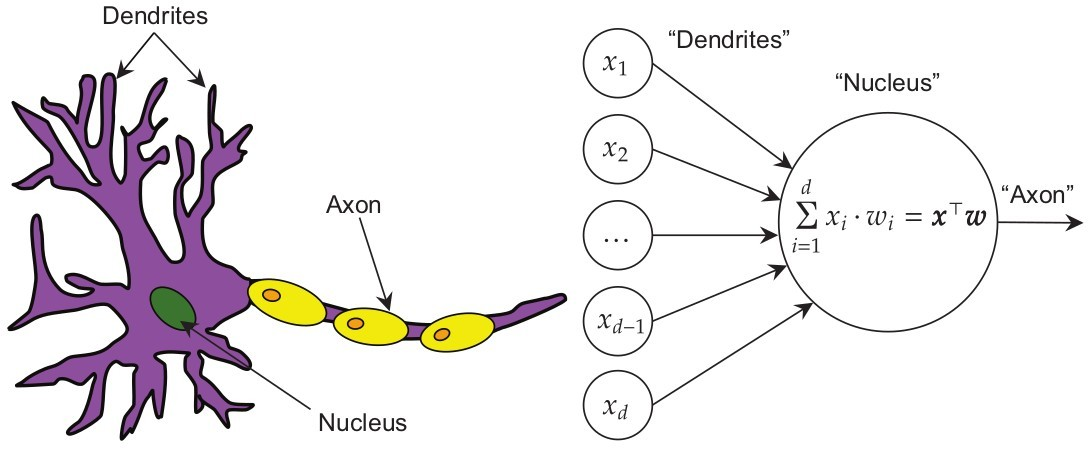
\includegraphics[width=0.8\textwidth]{img/neoantigen/neuron}
	\caption{Representación de una neurona. Fuente: \cite{insideDL2022}.}
	\label{fig:neuron}
\end{figure}

El perceptron, es capaz de solucionar varios problemas, pero para casos complejos puede formar una red, como se presenta en la Figura \ref{fig:nn}.

\begin{figure}[H]
	\centering
	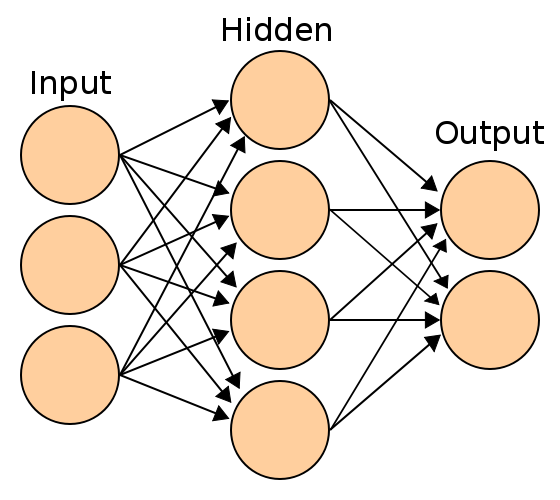
\includegraphics[width=0.35\textwidth]{img/neoantigen/nn2}
	\caption{Representación de una red neuronal. }
	\label{fig:nn}
\end{figure}

\section{\textit{Deep learning}}

\textit{Deep learning} (DL) es una subcategoría de \textit{Machine Learning}, a diferencia de los algoritmos tradicionales de ML, usualmente DL trata con señales sin pre-procesamiento, los modelos (basados en redes neuronales) son mucho mas complejos tanto en dimensión como en el método de aprendizaje \citep{el2022machine}. Por ejemplo, en la Figura \ref{fig:dl}, presentamos la relación entre inteligencia arficial, ML y DL, de ahí podemos concluir que ML es parte de la IA y DL es parte de ML \citep{el2022machine}.

\begin{figure}[H]
	\centering
	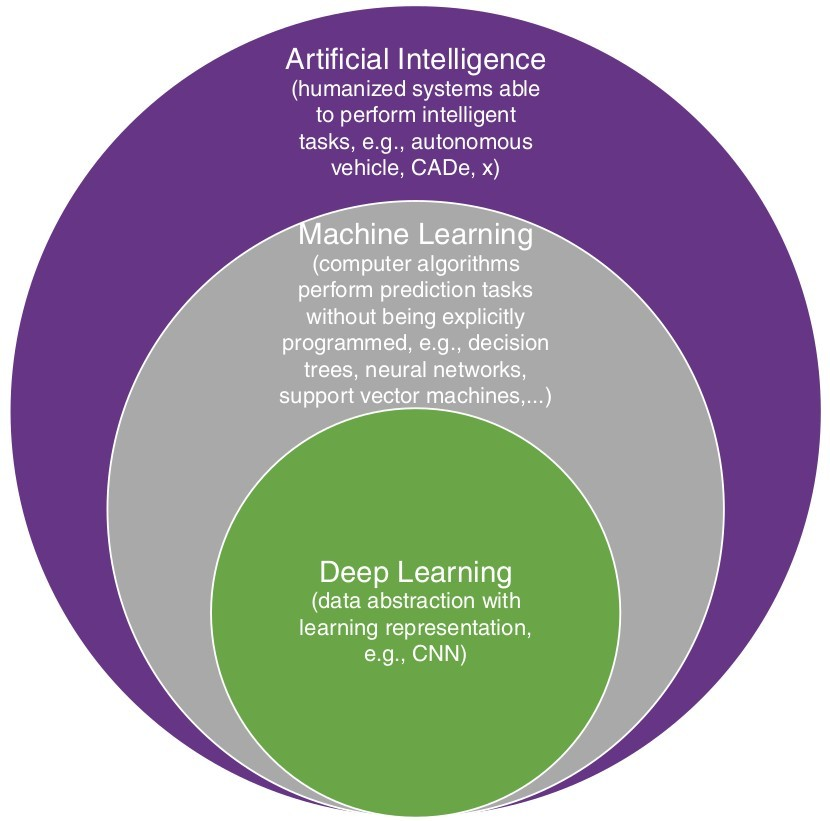
\includegraphics[width=0.5\textwidth]{img/neoantigen/dl}
	\caption{Relación entre Inteligencia Artificial, \textit{Machine Learning} y \textit{Deep Learning}. Fuente: \cite{el2022machine}.}
	\label{fig:dl}
\end{figure}


\subsection{\textit{Deep Feedforward networks}}

\textit{Deep Feedforward networks} son perceptrones multicapa o \textit{multilayer perceptrons}(MLP). Su objetivo es aproximar una función $f^*$, para el caso de clasificación, podría modelarse como $ y=f^*(x)$. Luego, un \textit{feedforward network}, define un mapeo $y = f(x;\theta)$ y aprende los valores de los parametros $\theta$ \cite{Goodfellow2016}. Entonces un \textit{Deep Feedforward networks}, es una red neuronal tradiconal pero con un número grande de neuronas y capas (Figura \ref{fig:dnn}). Existen muchos tipos de \textit{Deep Feedforward networks}, estas serán detalladas en los siguientes apartados.

\begin{figure}[H]
	\centering
	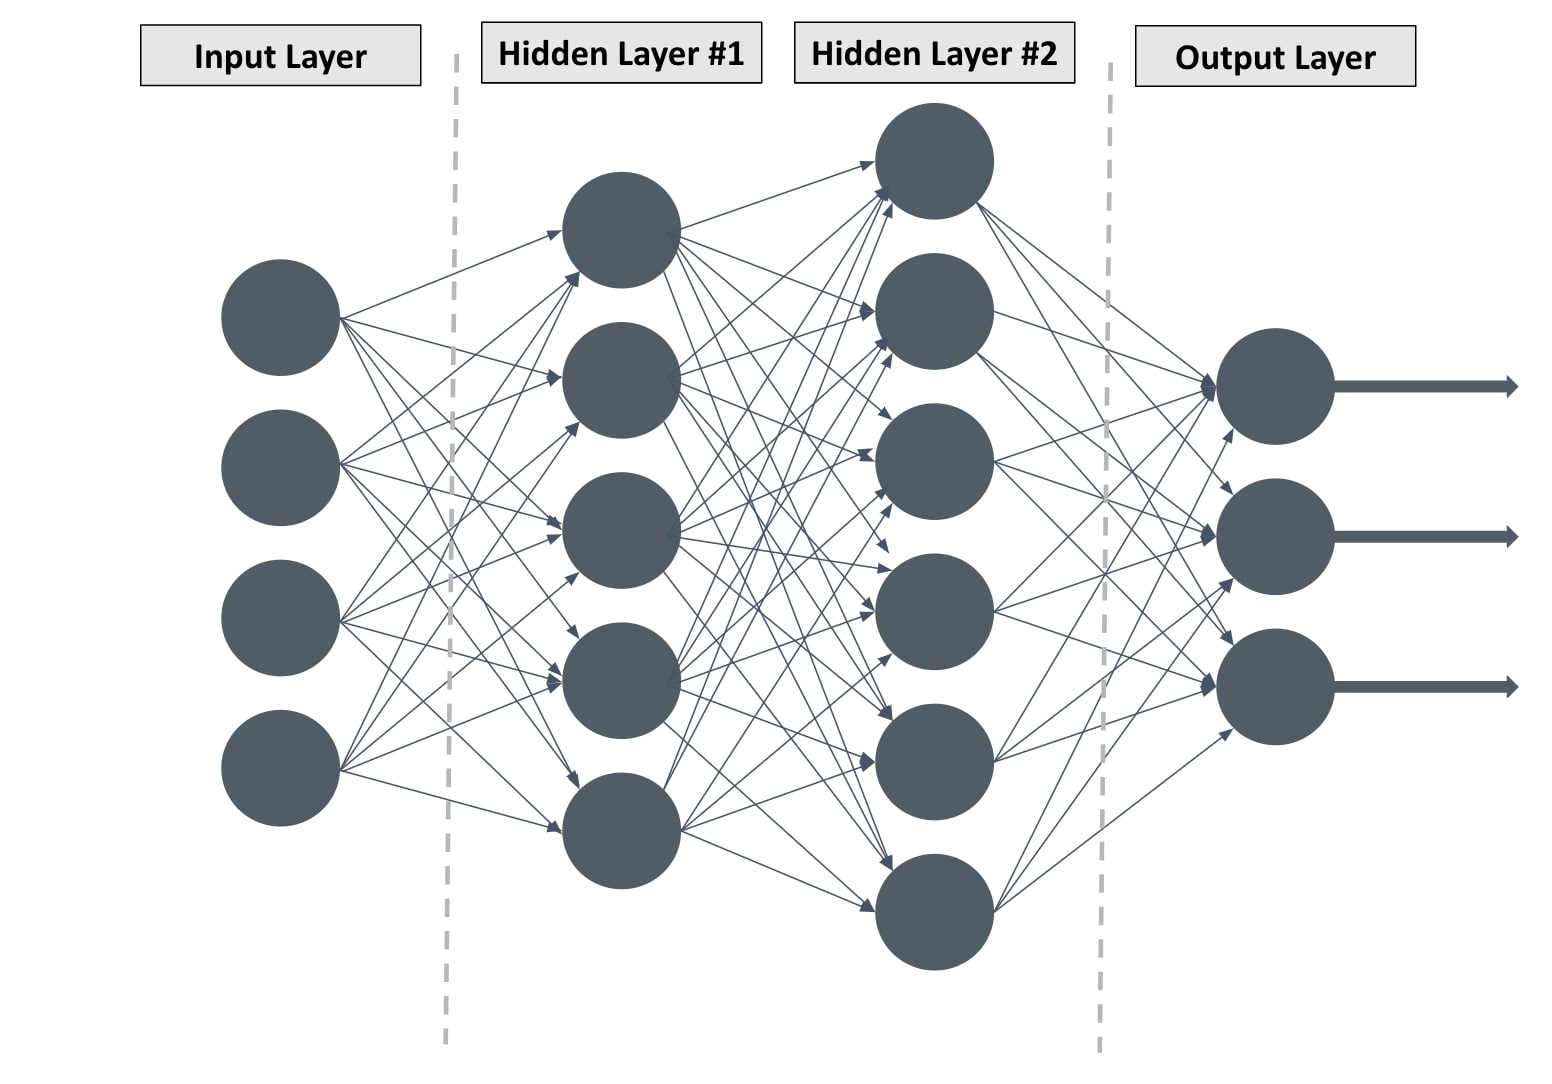
\includegraphics[width=0.7\textwidth]{img/neoantigen/deep_nn}
	\caption{Representación de un \textit{Deep Feedforward Network}. Fuente: \cite{el2022machine}.}
	\label{fig:dnn}
\end{figure}


\subsection{\textit{Convolutional Neural Networks}}

Una \textit{Convolutional Neural Networks} (CNN), es una red neuronal basada en la operación de convoluciones (utilizada en procesamiento de imágenes). Generalmente estas redes neuronales se aplican a problemas de visión computacional \citep{zhang2021dive}. La operación básica es la convolución, esta se presenta en la Figura \ref{fig:cnn}. Se toman pequeñas ventanas de una imagen y se realiza el producto punto con un \textit{kernel} ya establecido. Según los diferentes valores del \textit{kernel}, se pueden obtener diferentes resultados en la imagen de salida como: detección de bordes, suavizados, dilatación, etc.


\begin{figure}[H]
	\centering
	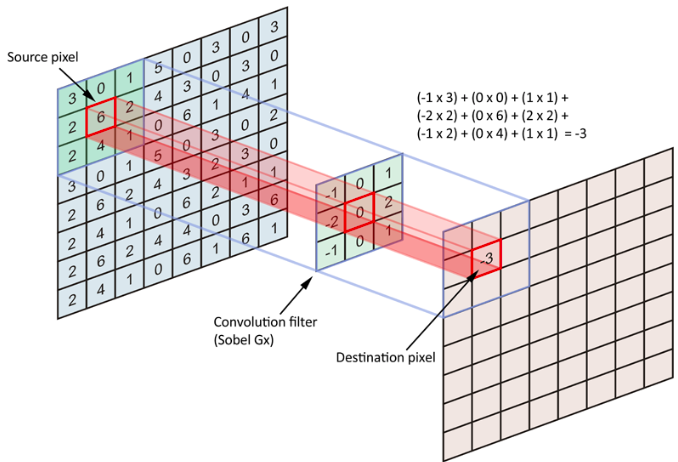
\includegraphics[width=0.7\textwidth]{img/neoantigen/cnn}
	\caption{Ejemplo de una convolución en procesamiento de imágenes. Fuente: \cite{Shuchen2022}.}
	\label{fig:cnn}
\end{figure}

Con inspiración en la operación de convolución, se plantean las CNN por primera vez por \cite{lecun1998gradient}. En la Figura \ref{fig:cnn3}, se presenta la LeNet-5, planteado por los autores. Luego, surgen diversa propuestas como AlexNet \citep{krizhevsky2012imagenet}, VGGNet \citep{simonyan2014very}, GoogleNet \citep{szegedy2015going} y ResNet \citep{he2016deep}.

\begin{figure}[H]
	\centering
	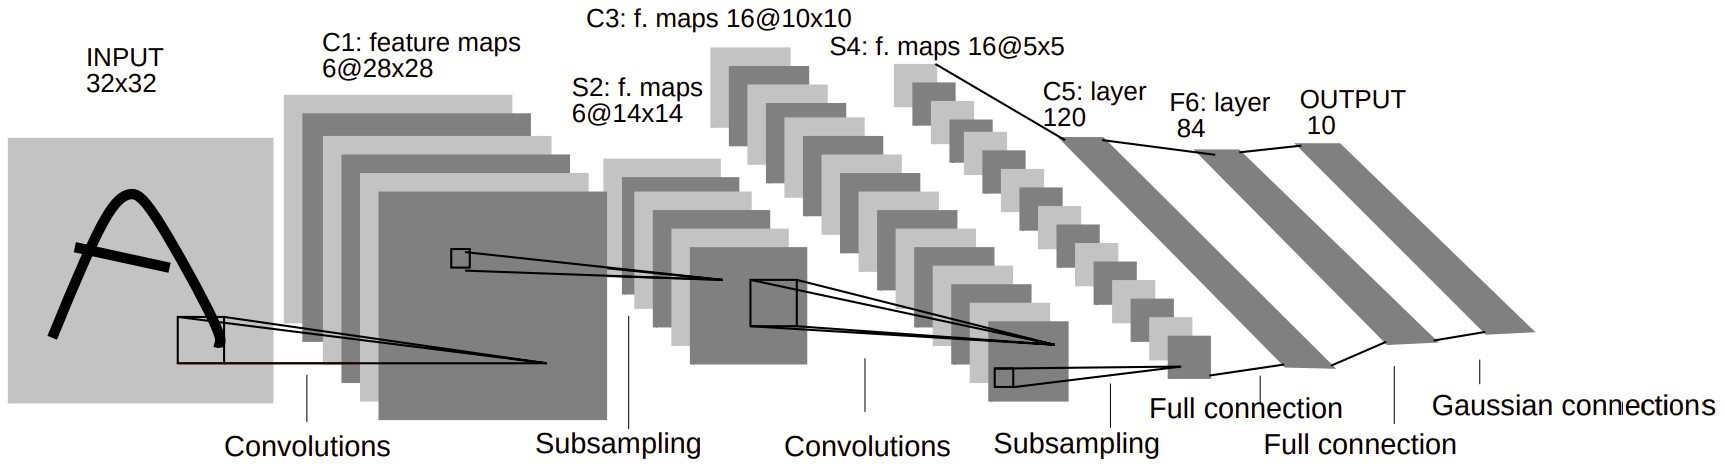
\includegraphics[width=\textwidth]{img/neoantigen/cnn3}
	\caption{Arquitectura de LeNet-5, una CNN para el reconocimiento de digitos. Fuente: \cite{lecun1998gradient}.}
	\label{fig:cnn3}
\end{figure}


\subsection{\textit{Recurrent Neural Networks}}

Mientras que las CNN están especializadas para manejar información espacial, las \textit{Recurrent Neural Networks} (RNN), se especializan en información secuencial  \citep{zhang2021dive}. En este campo, se habla del tiempo como una variable y se tratan problemas de series temporales por ejemplo.

El término RNN, aparece por primera vez en los trabajos de \cite{rumelhart1985learning} y \cite{jordan1997serial}. Algunos autores, comentan también que el inicio de las RNN fue con las redes de Hopfield  \citep{hopfield1982neural}. En general estas RNN, tienen dos entradas: estado actual y estado anterior; luego la RNN predice el siguiente estado. El problema de estas redes neuronales surgen por una falta de memoria, es decir cuando tenemos varios estados, el estado inicial va a influenciar cada vez menos a los estados futuros.

Como alternativa de solución al problema mencionado anteriormente, surgen Long Short-Term Memory, propuesta por \cite{hochreiter1997long}. Una red neuronal LSTM, es capaz de recordar un dato relevante de una secuencia y almacenarlo varios instantes de tiempo. En la Figura \ref{fig:lstm}, explicamos brevemente el funcionamiento de LSTM, los datos que ingresan a una compuerta (\textit{gate}), son los datos de entrada en un tiempo específico y el estado oculto anterior. Luego, es procesado por tres capas totalmente conectadas: \textit{input gate}, \textit{forget gate} y \textit{output gate} \citep{zhang2021dive}.

\begin{figure}[H]
	\centering
	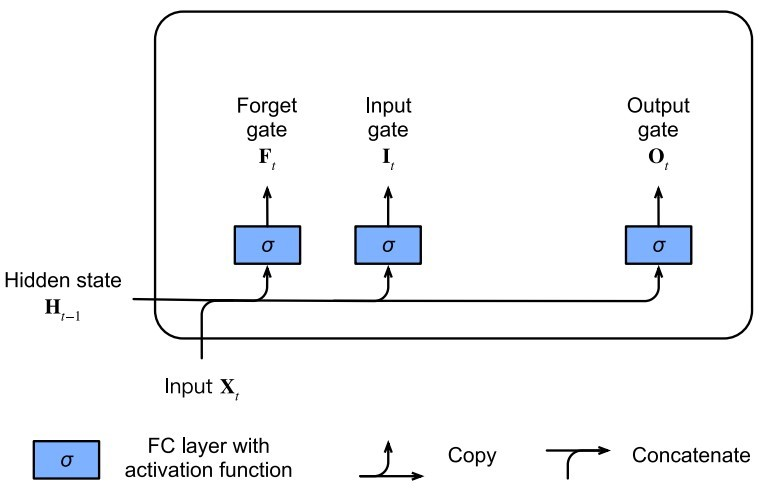
\includegraphics[width=0.7\textwidth]{img/neoantigen/lstm}
	\caption{Ejemplo del procesamiento del \textit{input gate}, \textit{forget gate} y \textit{output gate} de LSTM. Fuente: \cite{zhang2021dive}.}
	\label{fig:lstm}
\end{figure}

\subsection{\textit{Transformers}}

Los \textit{Transformers} son propuestas por \cite{vaswani2017attention}, para dar solución al problema de \textit{long-range dependency}. Por ejemplo el autor comenta: ``The Transformer is the first transduction model relying entirely on self-attention to compute representations of its input and output without using sequence-aligned RNNs or convolution''. Del enunciado anterior, \textit{transduction} hace referencia a la conversión secuencias de entrada hacia otro formato. Otro termino interesante es \textit{self-attention} (Figura \ref{fig:transformer}), este permite al modelo mirar hacia otras palabras en la secuencia de entrada para tener un mejor entendimiento de cierta palabra en la secuencia  \citep{Kelvin_transformer2022}.  

\begin{figure}[H]
	\centering
	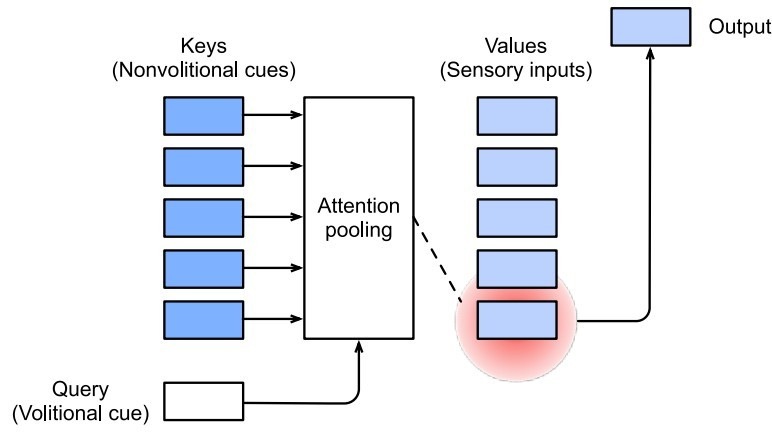
\includegraphics[width=0.7\textwidth]{img/neoantigen/transformer}
	\caption{ejemplo del mecanismo de atención de una red \textit{Transformer}. Fuente: \cite{zhang2021dive}.}
	\label{fig:transformer}
\end{figure}


\subsection{\textit{BERT}}

\textit{Bidirectional Encoder Representations from Transformers (BERT)}, propuesta por \cite{devlin2018bert}, está inspirada por la red \textit{Tranformer} y su mecanismo de atención, la cuál entiende la relación contextual entre diferentes palabras. A diferencia de una RNN, BERT no tiene dirección, es decir lee la secuencia entera. Esta característica, le permite al modelo aprender información contextual de una palabra con respecto a las otras \citep{Kelvin_transformer2022}.








%EOF
